\documentclass[17pt, t, lualatex]{beamer}



\title{\LARGE Cambio en los Ingresos de Familias Desplazadas del Meta por el Conflicto Armado: Metodología y Resultados}
\date{\today}
\institute[UJTL]{Universidad Jorge Tadeo Lozano}
\author{Ludwig Alvarado Becerra}

\usepackage{amsmath, amssymb, mathtools}
\usepackage[spanish]{babel}
\usepackage{biblatex}
\usepackage{hyperref}
\usepackage{xurl}
\usepackage{cancel}
\usepackage{svg}

\addbibresource{referencias.bib}  % Make sure your .bib file is correctly named


\addbibresource{referencias.bib}

% Probably load as late as possible
% Other options are
% - engine=pdflatex to compile in pdfLaTeX (with different fonts),
% - mathshape=rm to use serif font for math,
% - mathsahpe=custom to not set any math font (so that you can define your own math fonts)
\usetheme[engine=lualatex, mathshape=sf, fontdir=kthpq-files/fonts/Figtree/]{kthpq}
\setmonofont{Bitstream Vera Sans Mono}[Scale=.9]

% Custom colors (see beamercolorthemecustom.sty for more details)
% \usecolortheme{custom}

% Modify the headline template: KTH-full, KTH-section-only, or KTH-frametitle-only.
% \setbeamertemplate{headline}[KTH-full]

% Custom footline
% \setfootline{left}{center}{right}

\begin{document}

\inserttitlepage

\section{Recapitulación}

\insertsectionpage


\begin{frame}
  \frametitle{Recapitulación} 

\begin{columns}
  \begin{column}{.5\textwidth}
    \begin{itemize}
      \item Métodos de los campesinos para generar ingresos.
      \item Pendiente tener más métodos en la conversión de unidades.
      \item Crear clase \textit{GrupoArmado}.
      \item Funciones de probabilidad para modelar los datos.
    \end{itemize}
  \end{column}

  \begin{column}{.5\textwidth}
    \begin{figure}[ht]
      \centering
      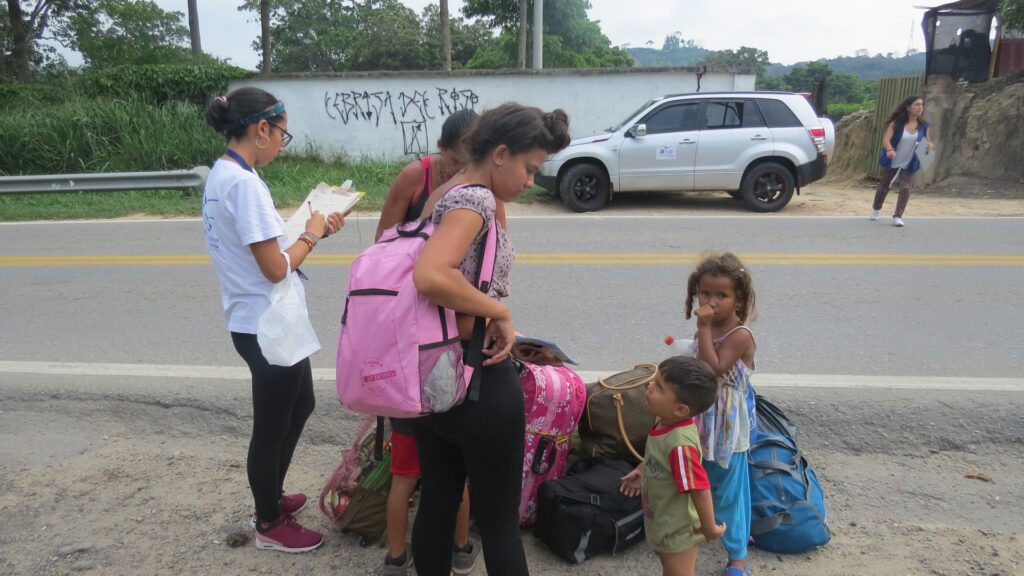
\includegraphics[width = 0.9\textwidth]{img/img1.jpg}
      \caption{Imagen sacada de \textit{Revista Cien Días, Persistencia del desplazamiento forzado y migración interna en Colombia}\cite{Leal2022Desplazamiento}.}
    \end{figure}

  \end{column}
\end{columns}


\end{frame}

\section{Modificación clase \textit{Campesino}}

\insertsectionpage

\begin{frame}
  \frametitle{Modificación clase \textit{Campesino}}


\begin{columns}
  \begin{column}{.5\textwidth}
  \begin{figure}[ht]
    \centering
    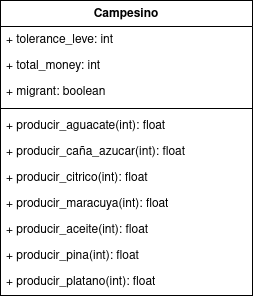
\includegraphics[width = 0.55\textwidth]{img/ClaseCampesino.png}
  \end{figure}  
  \end{column}

  \begin{column}{.5\textwidth}
\begin{figure}[ht]
    \centering
    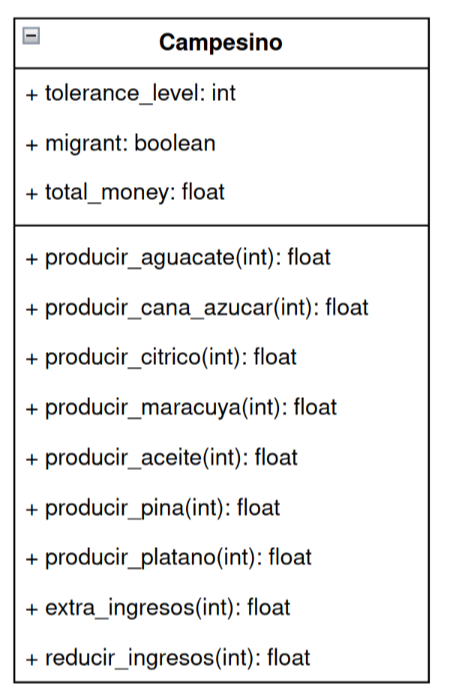
\includegraphics[width = 0.4\textwidth]{img/img2.png}
  \end{figure}
  \end{column}
\end{columns}
    


\end{frame}


\section{Creación clase \textit{GrupoArmado}}

\insertsectionpage

\begin{frame}
  \frametitle{Creación clase \textit{GrupoArmado}}
  \begin{figure}[ht]
    \centering
    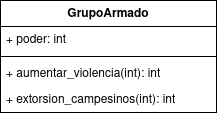
\includegraphics[width = 0.5\textwidth]{img/ClaseGrupoArmado.png}
  \end{figure}
\end{frame}

    
\section{Lógica (diagrama de flujo)}

\insertsectionpage

\begin{frame}
  \frametitle{Lógica (diagrama de flujo)}
  \begin{figure}[ht]
    \centering
    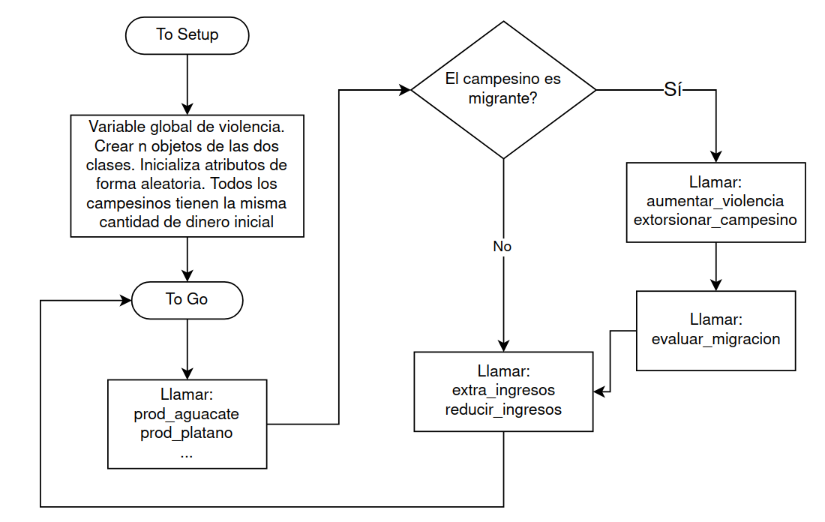
\includegraphics[width = 0.65\textwidth]{img/img3.png}
  \end{figure}
\end{frame}





\section{Resultados}

\insertsectionpage

\begin{frame}
  \frametitle{Paso 0}
  \begin{figure}[ht]
    \centering
    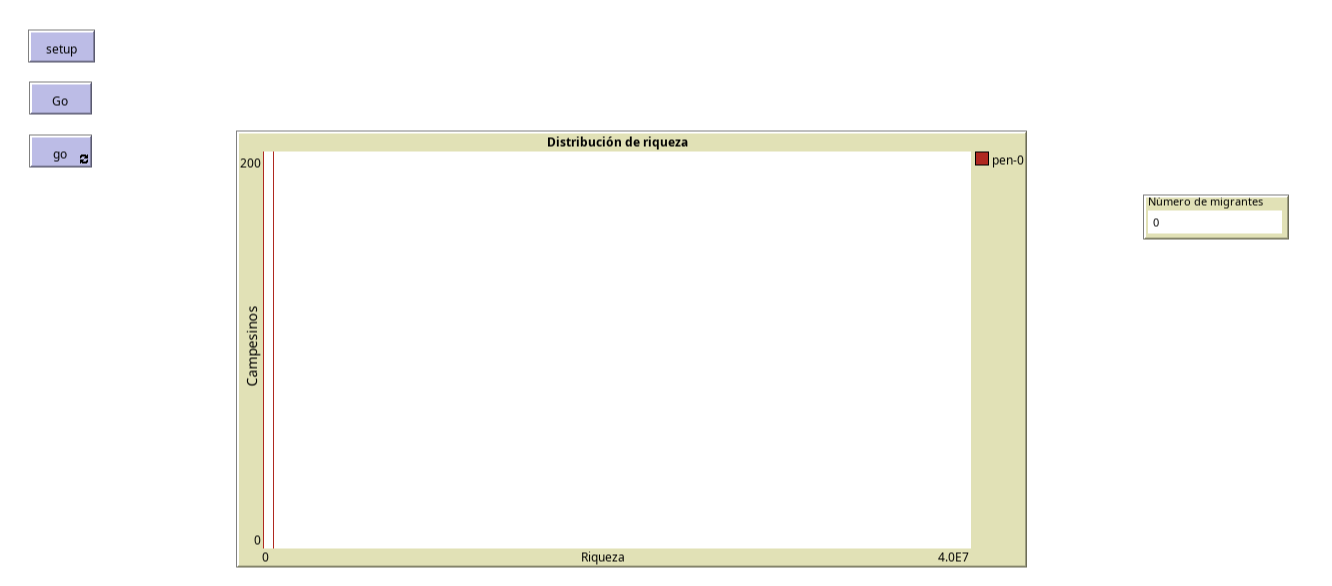
\includegraphics[width = 0.8\textwidth]{img/img4.png}
  \end{figure}
\end{frame}


\begin{frame}
  \frametitle{Paso 1}
  \begin{figure}[ht]
    \centering
    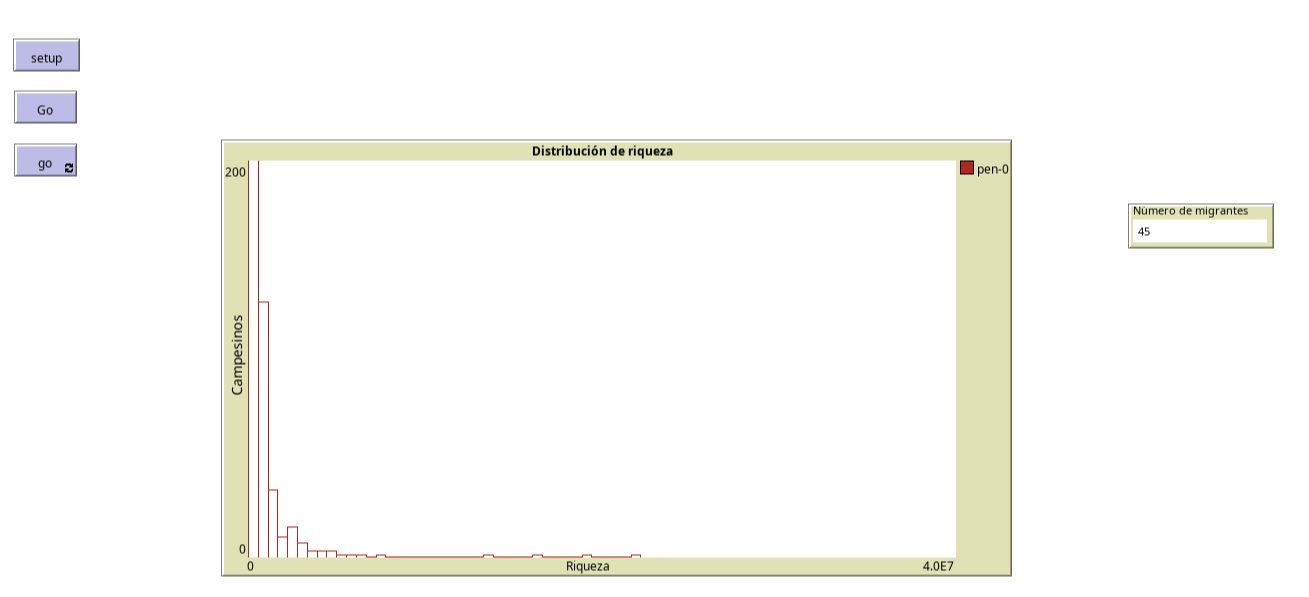
\includegraphics[width = 0.8\textwidth]{img/img5.png}
  \end{figure}
\end{frame}

\begin{frame}
  \frametitle{Paso 9}
  \begin{figure}[ht]
    \centering
    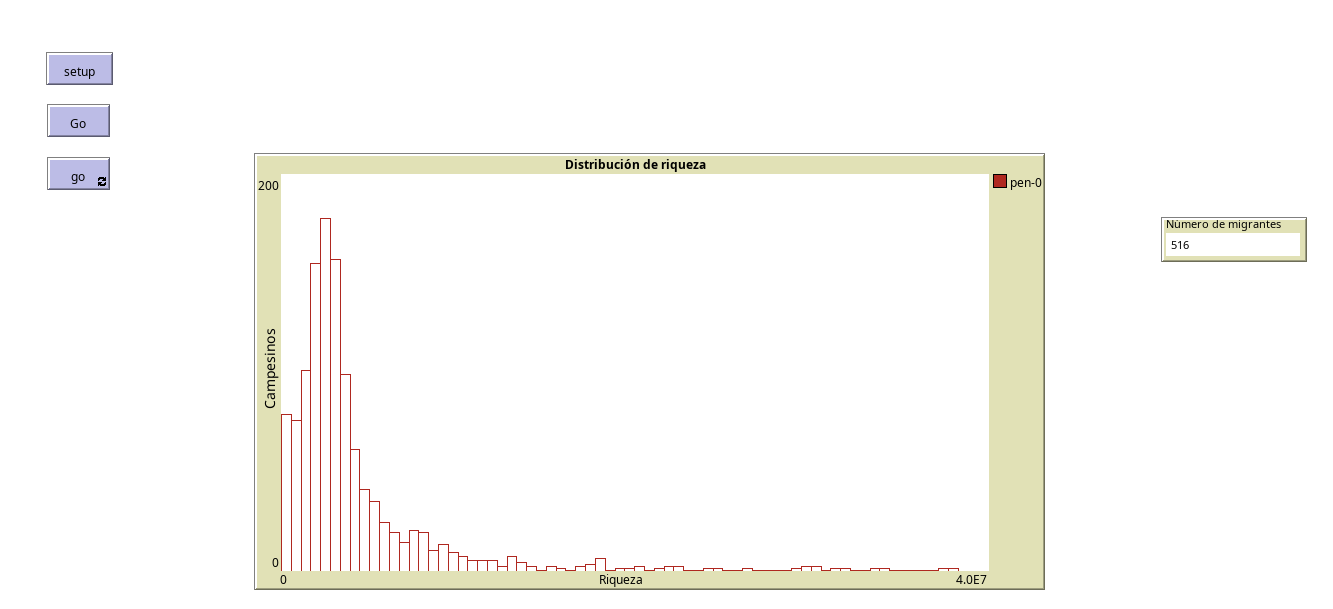
\includegraphics[width = 0.8\textwidth]{img/img6.png}
  \end{figure}
\end{frame}

\begin{frame}
  \frametitle{Paso 12}
  \begin{figure}[ht]
    \centering
    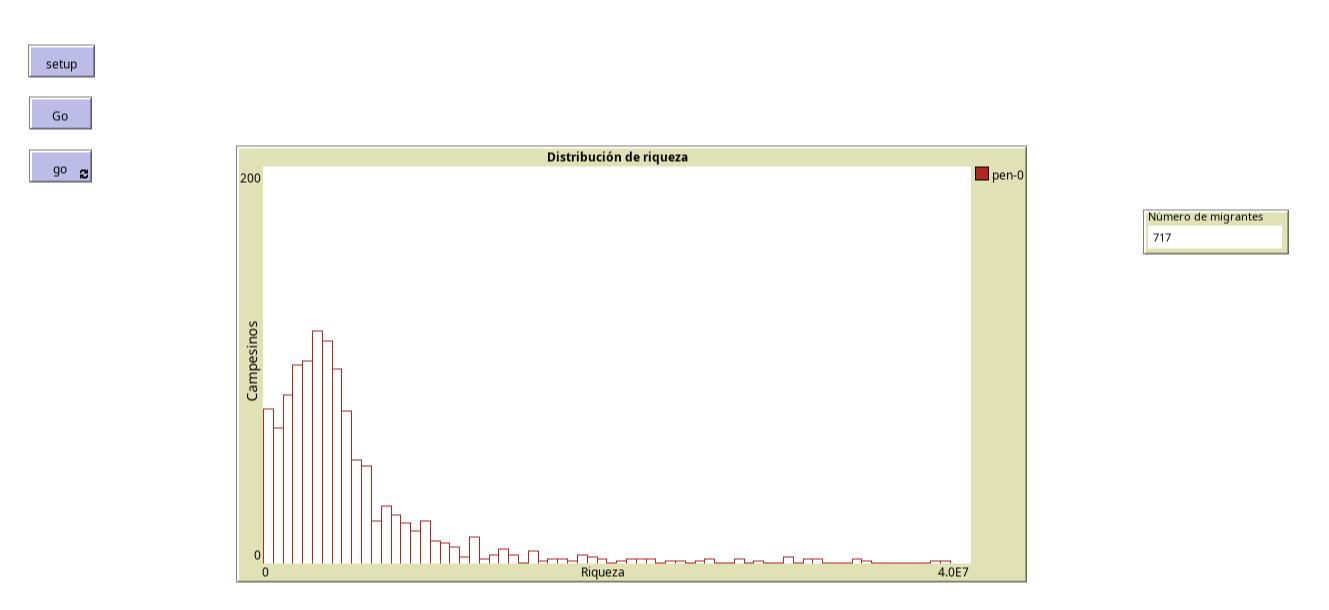
\includegraphics[width = 0.8\textwidth]{img/img7.png}
  \end{figure}
\end{frame}


\begin{frame}
  \frametitle{Paso 269}
  \begin{figure}[ht]
    \centering
    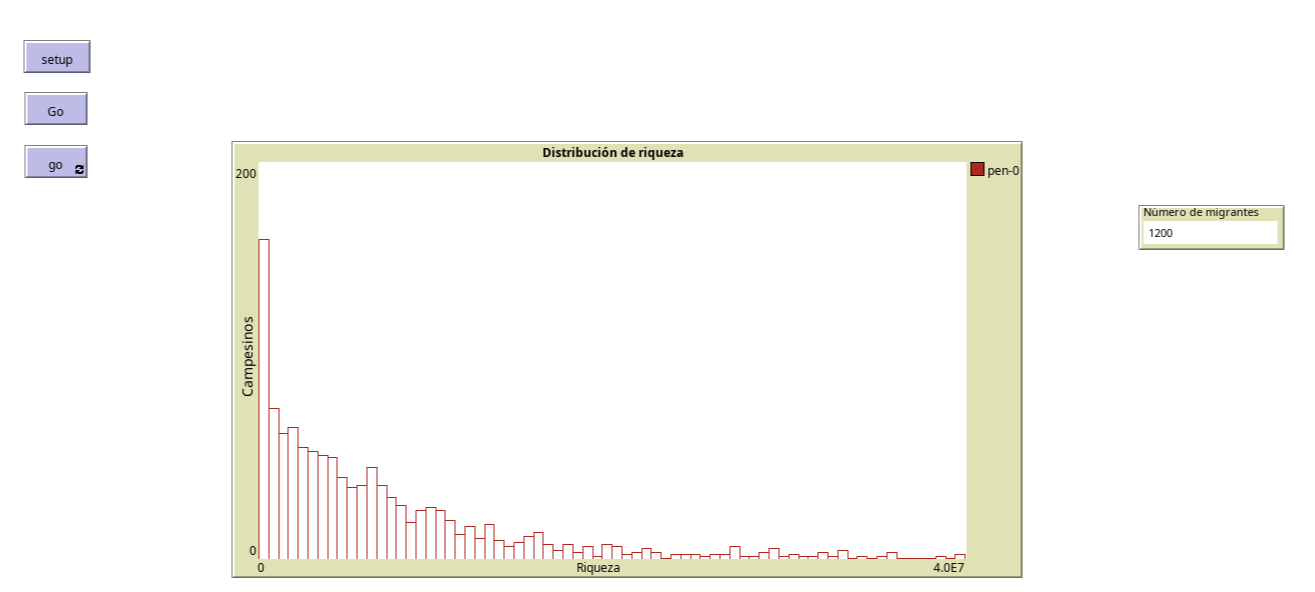
\includegraphics[width = 0.8\textwidth]{img/img8.png}
  \end{figure}
\end{frame}




\section{Conclusiones}

\insertsectionpage






\section{Licencia proyecto}

\insertsectionpage


\begin{frame}
  \frametitle{Licencia}

\begin{columns}
  \begin{column}{.5\textwidth}
    \begin{itemize}
      \item El código está bajo una licencia GPL V3, las presentaciones y escritos bajo la CC 4.0
      \item Todo el proyecto (bibliografía, avances, presentaciones y código) se encuentra en el siguiente enlace a \textit{GitHub} \url{https://github.com/TheLudway/abm-forced-displacement}
    \end{itemize}
  \end{column}

  \begin{column}{.5\textwidth}
    \begin{figure}[ht]
      \centering
      
\includegraphics[width = 0.7\textwidth]{img/gpl.png}
    \end{figure}

  \end{column}
\end{columns}


\end{frame}




\section{Referencias}

\insertsectionpage
\begin{frame}[allowframebreaks]{Referencias}
  \printbibliography
\end{frame}


\insertendpage

\end{document}
